\chapterheading{2}{CƠ SỞ LÝ THUYẾT}
\setcounter{section}{2}
\setcounter{subsection}{0}
\setcounter{subsubsection}{0}

\subsection{Thị giác máy tính và video giám sát}
\subsubsection{Khái niệm}
Thị giác máy tính là lĩnh vực nghiên cứu các phương pháp giúp máy tính trích xuất thông tin có cấu trúc từ ảnh và video. Trong bài toán của đồ án, đầu vào không phải một ảnh độc lập mà là chuỗi khung hình theo thời gian. Mỗi frame chứa thông tin vị trí tức thời; ý nghĩa ``nhân viên đang hiện diện'', ``đã rời khỏi khu vực'', hoặc ``đã sử dụng điện thoại 12 phút'' chỉ xuất hiện khi kết hợp nhiều frame và lưu lịch sử trạng thái.

Ảnh màu có thể biểu diễn bởi tensor $I\in\mathbb{R}^{H\times W\times C}$, với $H$, $W$ là chiều cao, chiều rộng và $C$ là số kênh màu. Video là chuỗi $V=\{I_t\}_{t=1}^{T}$, trong đó khoảng thời gian giữa hai frame phụ thuộc FPS. Nếu xử lý 25 FPS, một phút video tương ứng khoảng 1500 frame. Vì vậy thuật toán cần cân bằng giữa độ chính xác, độ trễ và tài nguyên tính toán.

\subsubsection{Pipeline video analytics}
Một pipeline giám sát video thường gồm bốn tầng: thu nhận, nhận thức, liên kết theo thời gian và suy luận nghiệp vụ. Thu nhận chịu trách nhiệm đọc RTSP/tệp camera và xử lý lỗi kết nối. Nhận thức tạo detection. Liên kết theo thời gian duy trì identity tạm thời của đối tượng. Tầng nghiệp vụ áp dụng quy tắc vùng, state machine và tổng hợp thời gian. Tách tầng giúp mỗi thành phần có thể kiểm thử độc lập và thay thế model mà không thay đổi toàn bộ hệ thống.

\subsection{Phát hiện đối tượng}
\subsubsection{Định nghĩa bài toán}
Object detection xác định đồng thời lớp và vị trí của nhiều đối tượng trong ảnh. Đầu ra thường là bộ:
\begin{equation}
 d_i=(b_i,c_i,s_i),
\end{equation}
trong đó $b_i=(x_1,y_1,x_2,y_2)$ là bounding box, $c_i$ là nhãn lớp và $s_i\in[0,1]$ là confidence. Theo tài liệu Ultralytics, detector trả về bounding box, class label và confidence cho các đối tượng được phát hiện \cite{ultralyticsdetect}.

Độ chồng lấn giữa hai box thường được đo bằng Intersection over Union:
\begin{equation}
 IoU(A,B)=\frac{|A\cap B|}{|A\cup B|}.
 \label{eq:iou}
\end{equation}
IoU được dùng trong đánh giá detection, non-maximum suppression và nhiều thuật toán tracking.

\subsubsection{YOLO và YOLOv8}
YOLO đặt bài toán phát hiện thành suy luận một lượt trên toàn ảnh. Phiên bản YOLO đầu tiên của Redmon và cộng sự nhấn mạnh tính thời gian thực bằng cách dự đoán trực tiếp bounding box và class probability từ ảnh đầu vào \cite{yolo}. Các phiên bản sau cải thiện backbone, neck, head, chiến lược gán mẫu và loss.

YOLOv8 do Ultralytics phát hành năm 2023. Ultralytics công bố YOLOv8 như một họ model hỗ trợ detection, segmentation, pose, OBB và classification; các weight detection chuẩn được huấn luyện trên COCO với 80 lớp \cite{ultralyticsv8}. YOLOv8 không có bài báo học thuật chính thức tương ứng; vì vậy báo cáo trích dẫn tài liệu/phần mềm Ultralytics thay vì gán nhầm một bài báo khác cho kiến trúc này.

Đồ án chọn YOLOv8n làm cấu hình khởi đầu vì mô hình nhỏ và phù hợp xử lý trực tuyến. Hai lớp được dùng trực tiếp là \textit{person} và \textit{cell phone}. COCO là tập dữ liệu lớn cho nhận dạng đối tượng trong cảnh tự nhiên; phiên bản nghiên cứu gốc chứa hàng trăm nghìn ảnh và hàng triệu instance, tạo nền tảng pretrained phổ biến cho các detector tổng quát \cite{coco}.

\subsubsection{Ngưỡng confidence và NMS}
Nếu ngưỡng confidence quá cao, detector bỏ sót người bị che một phần; nếu quá thấp, số false positive tăng. Với tracking, việc bỏ toàn bộ detection có score thấp có thể làm track bị đứt. Đây chính là động cơ của ByteTrack: thay vì chỉ liên kết detection confidence cao, thuật toán còn dùng các detection thấp hơn trong bước ghép thứ hai để phục hồi đối tượng thật \cite{bytetrack}.

Non-Maximum Suppression loại bỏ các box dư thừa của cùng đối tượng. Với tập box cùng lớp, box có score cao nhất được giữ; các box còn lại có IoU vượt ngưỡng sẽ bị loại. Trong ứng dụng nhiều người đứng gần nhau, NMS quá mạnh có thể làm mất người thật, nên tham số cần đánh giá trên góc camera mục tiêu.

\subsection{Theo dõi đa đối tượng}
\subsubsection{Bài toán MOT}
Multi-Object Tracking nhận chuỗi detection và gán identity nhất quán cho các đối tượng qua thời gian. Mục tiêu không chỉ tìm đúng box mà còn duy trì quỹ đạo. Một tracker tốt phải hạn chế ba nhóm lỗi: bỏ sót/false positive, sai vị trí và sai association. HOTA được đề xuất để cân bằng chất lượng detection và association thay vì chỉ nhấn mạnh một thành phần \cite{hota}.

Trong tracking-by-detection, detector xử lý từng frame độc lập; tracker dự đoán vị trí của track ở frame sau và giải bài toán gán giữa track và detection. Hai thành phần kinh điển là Kalman filter cho dự đoán trạng thái và Hungarian algorithm cho assignment tối ưu. SORT kết hợp hai kỹ thuật này với IoU và cho thấy tốc độ theo dõi rất cao trong thiết lập trực tuyến \cite{sort}.

\subsubsection{Deep SORT}
SORT có thể đổi ID khi hai người che nhau hoặc quỹ đạo gần nhau. Deep SORT bổ sung embedding ngoại hình, dùng khoảng cách appearance kết hợp motion gating. Bài báo Deep SORT báo cáo giảm identity switch đáng kể so với SORT trên tập đánh giá của họ \cite{deepsort}. Đổi lại, hệ thống cần thêm một mạng re-identification và chi phí tính toán.

\subsubsection{ByteTrack}
ByteTrack quan sát rằng detection score thấp không đồng nghĩa với background; nhiều box score thấp là đối tượng thật bị che khuất. Thuật toán trước tiên liên kết track với detection score cao, sau đó tiếp tục liên kết các track chưa ghép với detection score thấp phù hợp. Những box thấp không khớp track được loại như background. Cách tiếp cận này giữ kiến trúc đơn giản nhưng cải thiện khả năng duy trì track qua che khuất \cite{bytetrack}.

Đối với đồ án, ByteTrack có ba ưu điểm: tích hợp thuận lợi với detector YOLO, không bắt buộc chạy mạng ReID toàn thân riêng, và tập trung đúng lỗi thường gặp trong CCTV là detection suy giảm tạm thời. Ultralytics cũng cung cấp cấu hình ByteTrack cho chế độ theo dõi video, cho phép dùng cùng model detection trong pipeline \cite{ultralyticstrack}.

\subsubsection{Track ID và danh tính nhân viên}
Track ID không phải employee ID. Track ID có vòng đời ngắn và có thể đổi khi đối tượng biến mất lâu. Vì vậy hệ thống duy trì ánh xạ:
\begin{equation}
 track\_id \rightarrow work\_area \rightarrow employee\_candidate \rightarrow identity\_state.
\end{equation}
Trong đó ROI cung cấp ngữ cảnh không gian; FaceNet chỉ hỗ trợ xác minh khi ảnh mặt đủ chất lượng. Tách hai loại định danh giúp tránh lỗi thiết kế phổ biến là lưu track ID như danh tính bền vững.

\subsection{Vùng quan tâm và hình học không gian ảnh}
\subsubsection{Biểu diễn polygon ROI}
Mỗi khu vực làm việc được biểu diễn bởi đa giác $A=\{v_1,\ldots,v_k\}$ trên hệ tọa độ ảnh. Polygon linh hoạt hơn rectangle vì camera phối cảnh khiến bàn và vùng sàn thường không song song với biên ảnh. Thao tác quản trị lưu các điểm theo tỉ lệ chuẩn hóa $(x/W,y/H)$ để khi thay đổi độ phân giải vẫn phục hồi được polygon tương ứng.

\subsubsection{Điểm neo của người}
Tâm bounding box có thể nằm phía trên bàn dù chân người ở ngoài ROI. Bởi vậy hệ thống dùng bottom-center như phương trình \ref{eq:anchor}. Đây là một xấp xỉ hình học: với camera cố định và người đứng/ngồi tương đối thẳng, đáy box gần giao điểm giữa cơ thể và mặt phẳng sàn hơn tâm box.

\subsubsection{Point-in-polygon}
Bài toán kiểm tra điểm nằm trong đa giác có thể giải bằng ray casting hoặc winding number. Trong cài đặt Python, có thể dùng thuật toán hình học tự cài đặt hoặc hàm thư viện như \texttt{cv2.pointPolygonTest}. Kết quả không nên áp dụng cứng ở đúng đường biên; hệ thống có thể dùng vùng đệm hoặc yêu cầu tỉ lệ quan sát trong ROI đủ lớn để tránh dao động khi người đứng sát biên.

\subsubsection{Chuyển vùng và cạnh tranh vùng}
Một track có thể đồng thời chạm hai ROI lân cận nếu dùng bounding box overlap. Khi đó, hệ thống ưu tiên ROI chứa bottom-center; nếu vẫn không duy nhất, dùng khoảng cách đến tâm/vùng lõi và trạng thái vùng trước đó. Hysteresis không gian giúp giảm việc track nhảy qua lại giữa hai khu vực khi đứng gần ranh giới.

\begin{figure}[H]
\centering
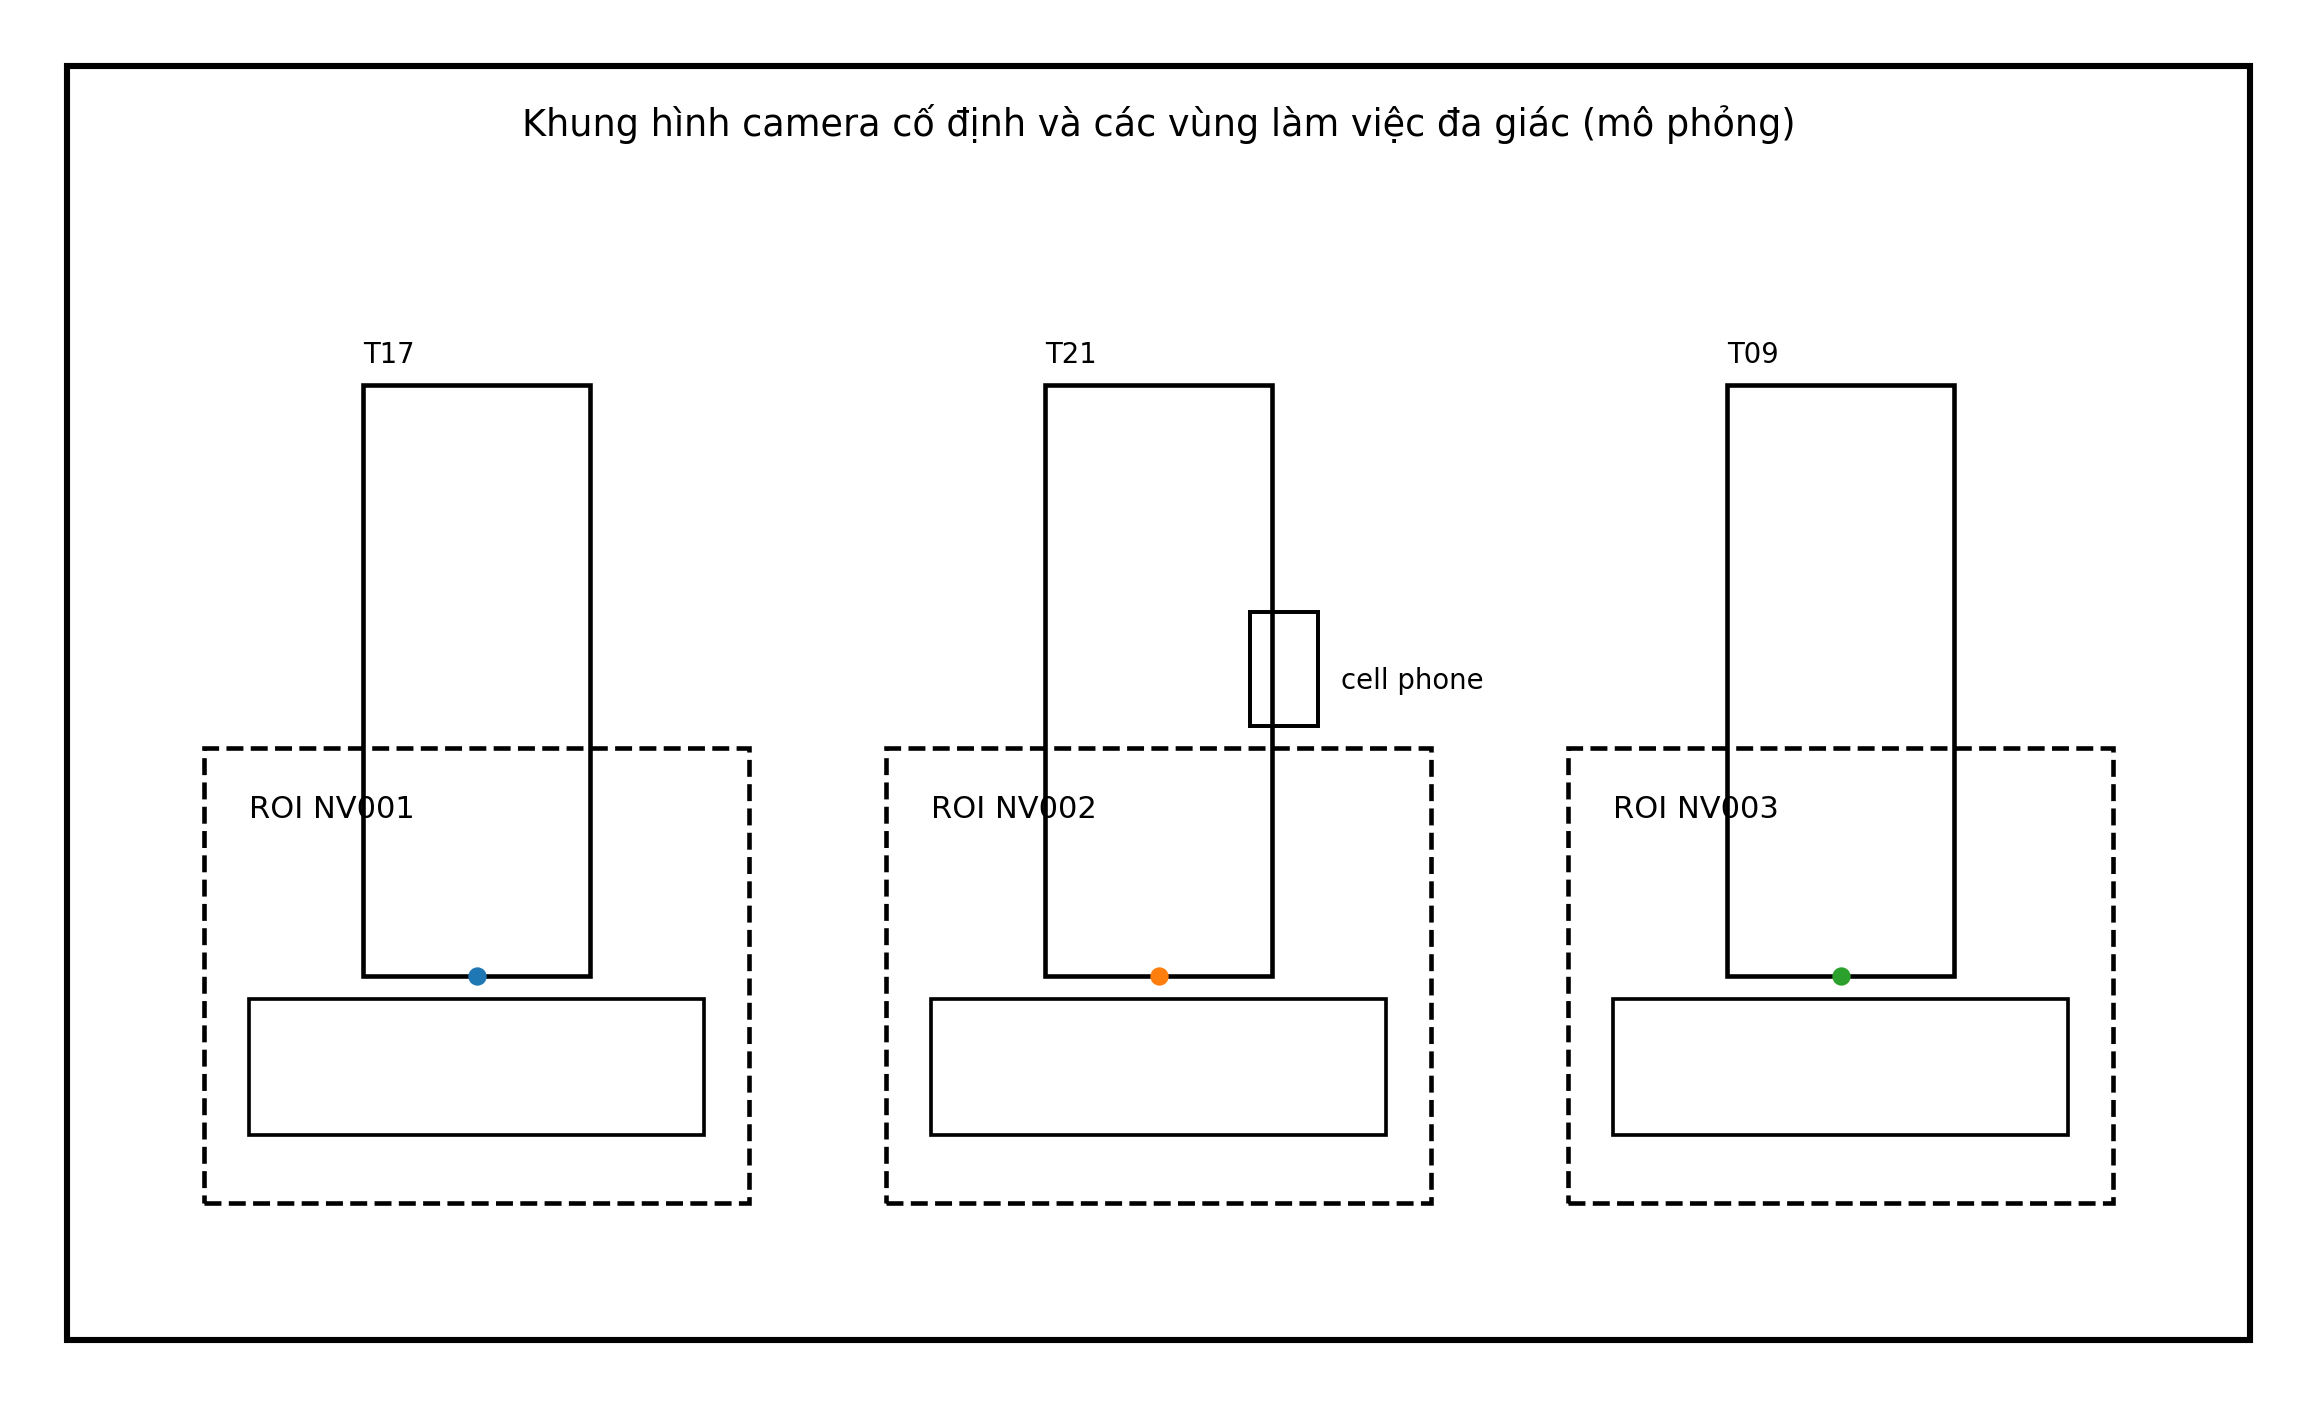
\includegraphics[width=0.92\textwidth]{Images/roi_scene.png}
\caption{Minh họa camera CCTV, nhiều track và vùng làm việc ROI}
\label{fig:roi-scene}
\end{figure}

\subsection{Xác thực danh tính bằng face embedding}
\subsubsection{Face embedding}
Face embedding ánh xạ ảnh khuôn mặt sang vector đặc trưng sao cho ảnh cùng người có khoảng cách nhỏ hơn ảnh khác người. FaceNet học không gian embedding trực tiếp và sử dụng triplet loss để kéo cặp cùng danh tính lại gần, đẩy danh tính khác ra xa \cite{facenet}.

Với hai embedding $u$ và $v$, cosine similarity là:
\begin{equation}
 sim(u,v)=\frac{u\cdot v}{\|u\|_2\|v\|_2}.
\end{equation}
Nếu embedding đã chuẩn hóa L2, cosine similarity thuận tiện để so sánh nhanh. Ngưỡng không nên lấy cố định từ một nghiên cứu khác mà phải hiệu chỉnh trên camera/điều kiện mục tiêu vì kích thước mặt, góc và ánh sáng thay đổi.

\subsubsection{Phát hiện và crop khuôn mặt}
Để lấy embedding, hệ thống cần face detector. MTCNN là mô hình cascade đa nhiệm phát hiện mặt và landmark, được đề xuất bởi Zhang và cộng sự \cite{mtcnn}. Trong source nền, MTCNN và InceptionResnetV1 của facenet-pytorch đã được sử dụng. Ở đề tài mới, MTCNN chỉ phục vụ bước xác minh identity theo sự kiện chứ không còn là detector chính của pipeline.

\subsubsection{Trạng thái identity}
Thay vì Boolean match/mismatch, đồ án dùng bốn trạng thái:
\begin{itemize}
\item \textbf{PROVISIONAL}: track mới nằm đúng ROI nhưng chưa có khuôn mặt đủ chất lượng.
\item \textbf{VERIFIED}: embedding đủ số quan sát và similarity vượt ngưỡng xác minh.
\item \textbf{UNKNOWN}: không đủ dữ liệu để kết luận.
\item \textbf{MISMATCH}: có đủ bằng chứng khuôn mặt nhưng không phù hợp nhân viên được gán.
\end{itemize}
Việc biểu diễn không chắc chắn giúp tránh biến lỗi camera thành kết luận sai về người lao động.

\subsection{Phát hiện và liên kết hành vi sử dụng điện thoại}
\subsubsection{Phát hiện điện thoại}
Lớp \textit{cell phone} nằm trong COCO, vì vậy YOLOv8 pretrained có thể tạo detection điện thoại cùng lúc với person. Tuy nhiên detection không chứng minh hành vi sử dụng. Điện thoại nằm trên bàn, trong tay người khác hoặc ở nền đều có thể xuất hiện.

\subsubsection{Vùng tương tác người--điện thoại}
Với person box $B_p$ và phone box $B_h$, hệ thống tạo một interaction region quanh phần thân trên và vùng phía trước của person. Các đặc trưng liên kết gồm: khoảng cách giữa tâm phone và tâm/điểm tay ước lượng của person, phone có nằm trong box mở rộng hay không, IoU với box person và quan hệ phone với ROI hiện tại. Một score tổng hợp có thể viết:
\begin{equation}
 S(p,h)=\alpha S_{dist}+\beta S_{contain}+\gamma S_{roi},
 \label{eq:phoneassoc}
\end{equation}
trong đó các thành phần được chuẩn hóa về $[0,1]$. Phone chỉ được gán cho người có score lớn nhất khi vượt ngưỡng; nếu hai score gần nhau hoặc đều thấp, owner được đặt UNKNOWN.

\subsubsection{Tại sao phải xử lý theo thời gian}
Một detection phone kéo dài 1--2 frame có thể là nhiễu. Ngược lại, điện thoại có thể bị tay che vài frame trong khi người vẫn đang sử dụng. Máy trạng thái theo thời gian có hai ngưỡng vào/ra giúp hấp thụ cả hai trường hợp. Đây là ý tưởng tương tự hysteresis: điều kiện để xác nhận bắt đầu cần mạnh hơn điều kiện duy trì.

\subsection{Xử lý tín hiệu theo thời gian}
\subsubsection{Debounce theo thời lượng}
Debounce trong ngữ cảnh này là yêu cầu tín hiệu duy trì đủ lâu trước khi chuyển trạng thái. Nếu $z(t)\in\{0,1\}$ là quan sát, điều kiện vào có thể viết:
\begin{equation}
 \int_{t-T_{enter}}^t z(\tau)d\tau \geq \rho T_{enter},
\end{equation}
trong đó $\rho$ là tỉ lệ quan sát hợp lệ tối thiểu. Triển khai rời rạc có thể dùng deque theo timestamp thay vì giả định FPS cố định.

\subsubsection{Cửa sổ thời gian trượt}
Cửa sổ trượt chỉ giữ các quan sát trong khoảng $[t-W,t]$. Tỉ lệ hiện diện:
\begin{equation}
 r(t)=\frac{N_{present}(t-W,t)}{N_{valid}(t-W,t)}.
\end{equation}
Nếu camera mất frame hoặc detector lỗi, mẫu không hợp lệ không nên tự động được xem là absent; cần phân biệt ``không thấy người'' và ``không có dữ liệu tin cậy''.

\subsubsection{Máy trạng thái hữu hạn}
Finite State Machine biểu diễn rõ các trạng thái và điều kiện chuyển. Với presence, các trạng thái ABSENT, CANDIDATE, PRESENT, GRACE giúp xử lý quá trình vào/ra. Với phone, NO\_PHONE, CANDIDATE, USING, GRACE có ý nghĩa tương tự. So với một chuỗi if-elif theo frame, FSM làm cho logic dễ kiểm thử, có thể lưu transition và tái dựng timeline.

\begin{figure}[H]
\centering
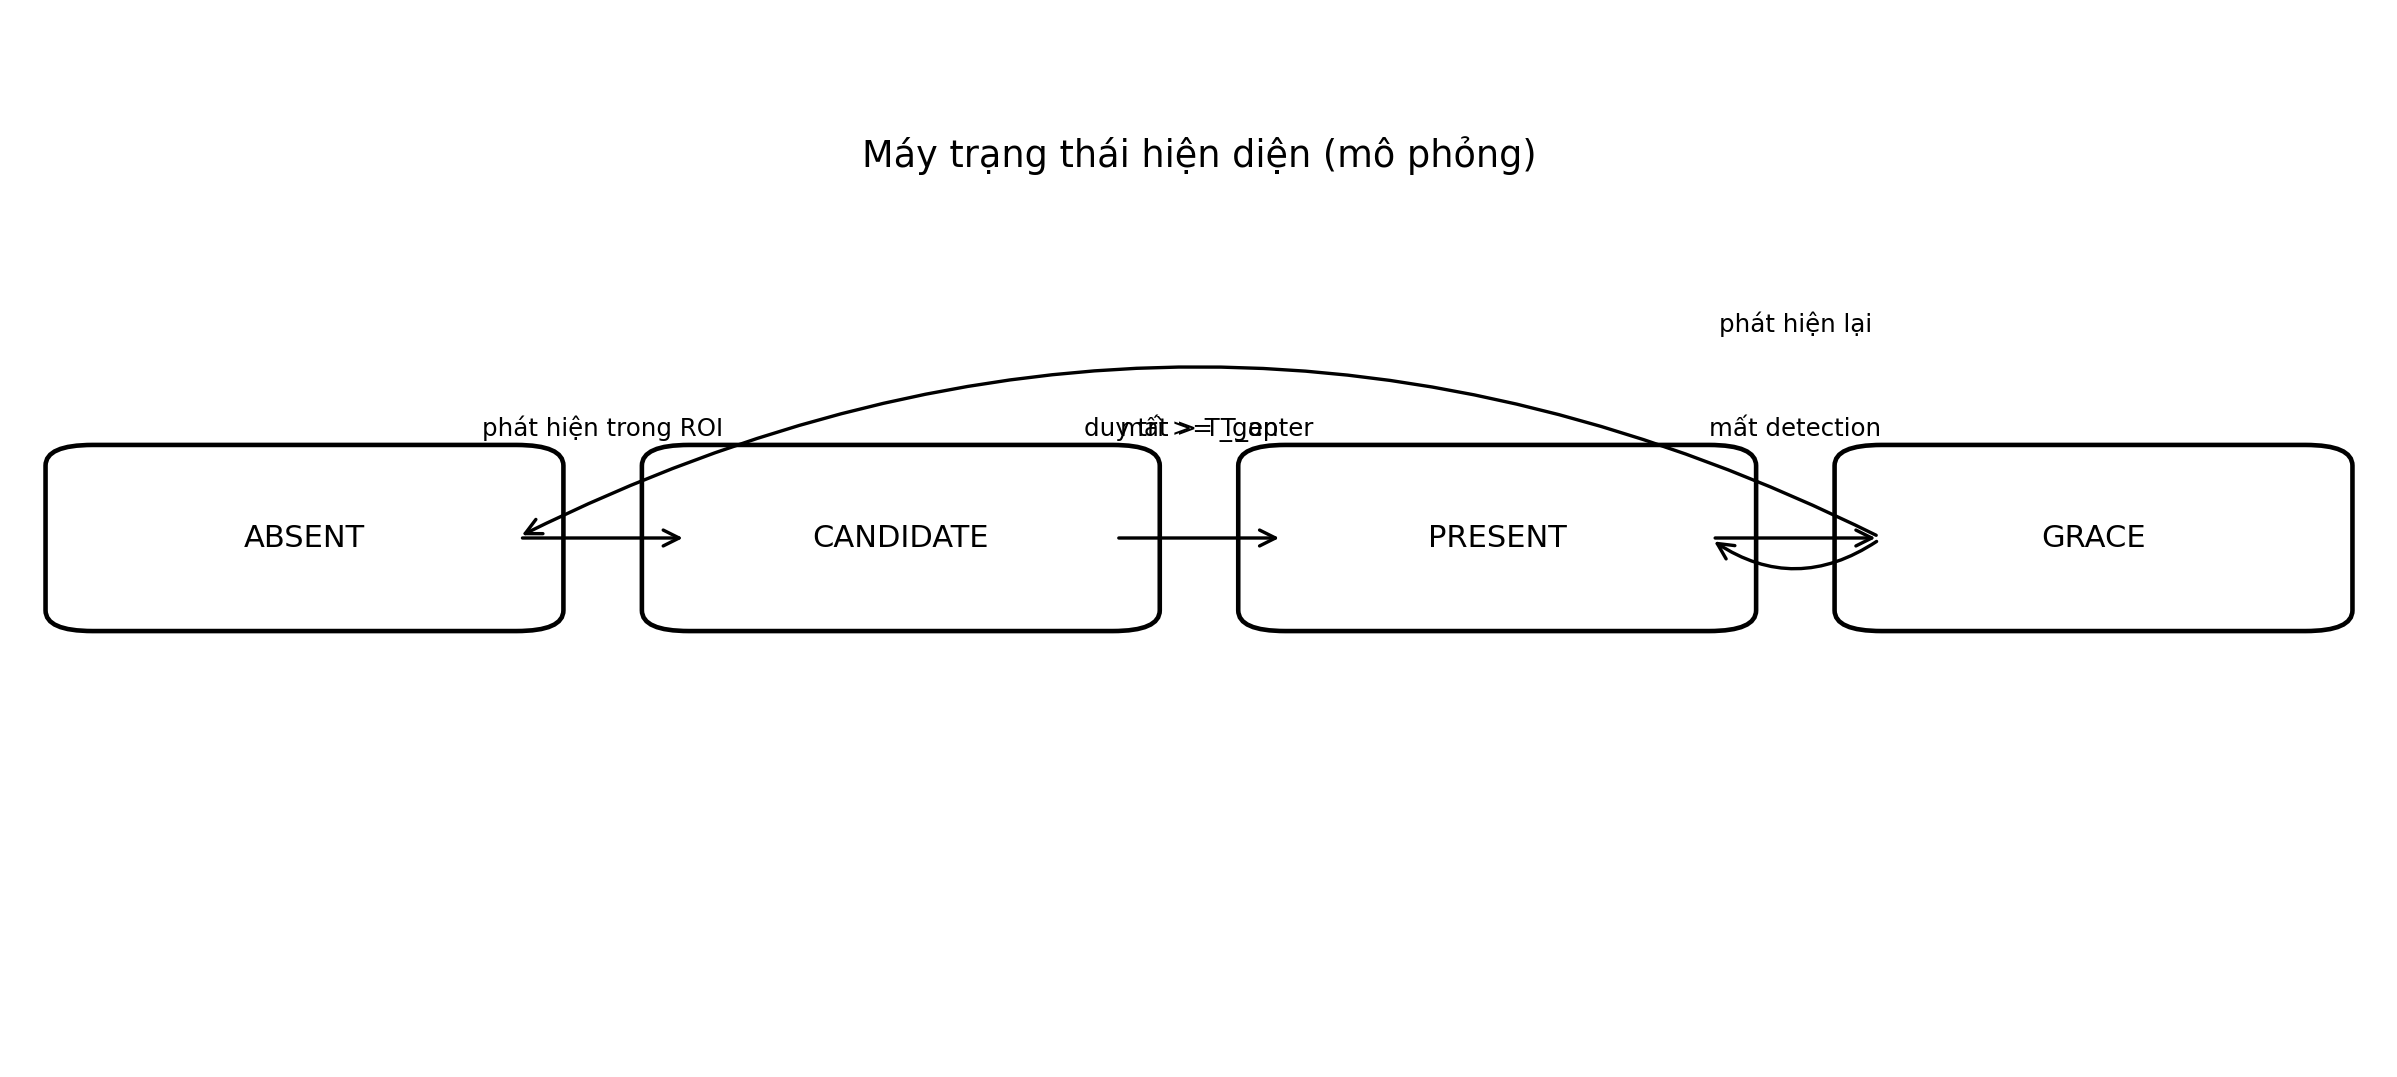
\includegraphics[width=0.95\textwidth]{Images/presence_state.png}
\caption{Máy trạng thái hiện diện đề xuất}
\label{fig:presence-state-theory}
\end{figure}

\begin{figure}[H]
\centering
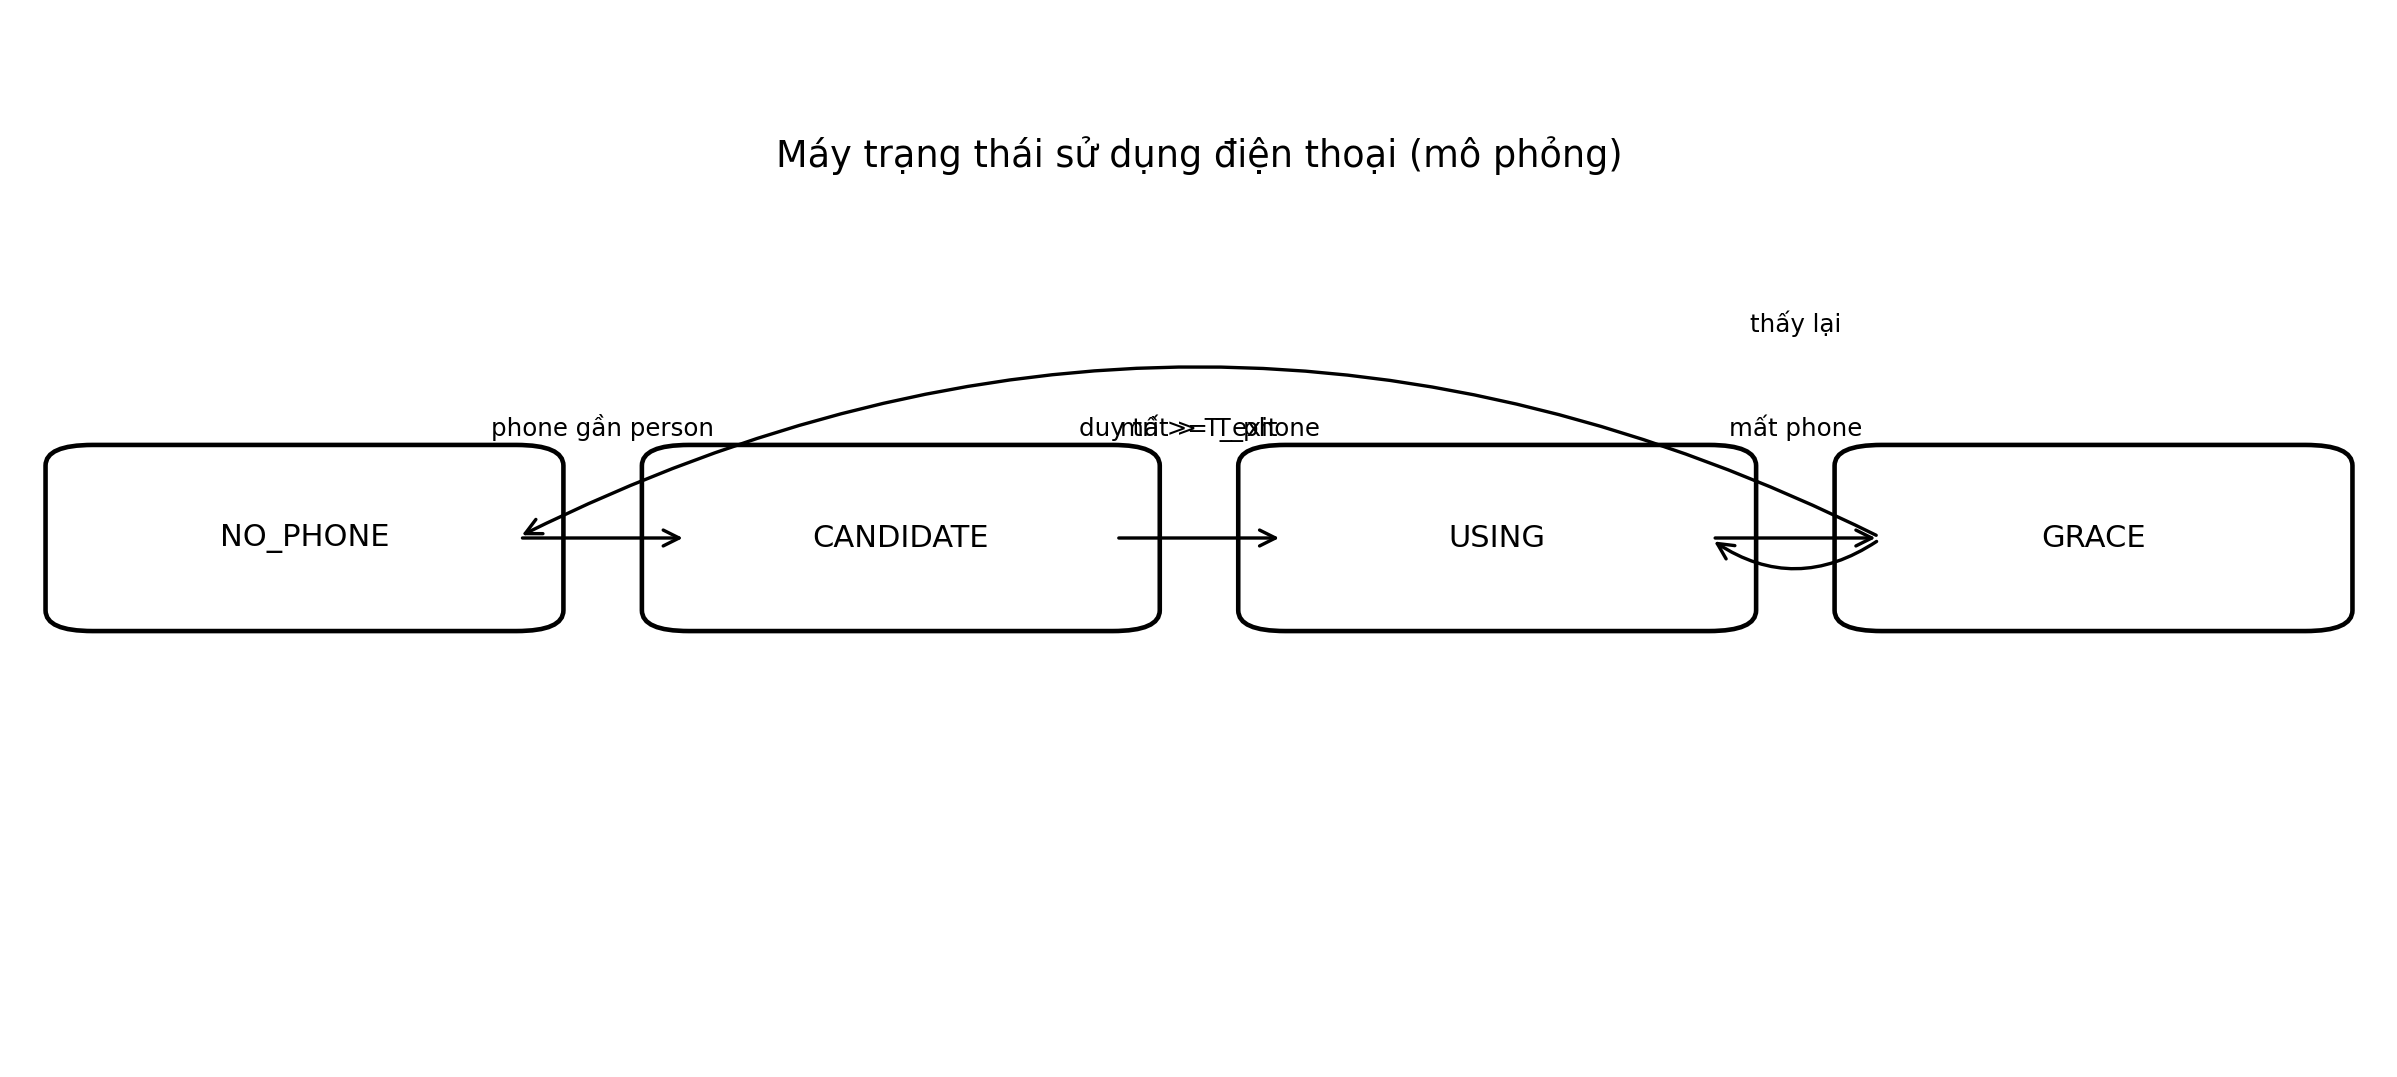
\includegraphics[width=0.95\textwidth]{Images/phone_state.png}
\caption{Máy trạng thái sử dụng điện thoại đề xuất}
\label{fig:phone-state-theory}
\end{figure}

\subsubsection{Hysteresis thời gian}
Nếu cùng một ngưỡng được dùng cho vào và ra, trạng thái có thể bật/tắt liên tục quanh biên. Hysteresis dùng $T_{enter}$ khác $T_{exit}$ hoặc tỉ lệ vào/ra khác nhau. Trong presence, hệ thống có thể yêu cầu 2 giây ổn định để xác nhận vào nhưng cho phép grace 5 giây khi mất detection. Mốc thời gian interval vẫn được neo về detection đầu tiên/last-seen để không tạo bias 2 hoặc 5 giây cho mọi phiên.

\subsection{Tổng hợp thời gian làm việc}
\subsubsection{Presence interval}
Một presence interval là cặp $(s,e)$ đã qua xác nhận temporal. Khi chuyển từ CANDIDATE sang PRESENT, hệ thống ghi $s$ là thời điểm ứng viên đầu tiên đủ điều kiện lịch sử. Khi GRACE chuyển sang ABSENT, $e$ là last-seen đáng tin cậy. Cách backdating giúp state machine lọc nhiễu mà không làm thay đổi tổng thời gian chỉ vì có ngưỡng xác nhận.

\subsubsection{Giao với lịch làm việc}
Nếu ca làm là tập cửa sổ $W=\cup_l[a_l,b_l]$, thời gian hiện diện hợp lệ là tổng giao giữa presence intervals và $W$. Khoảng nghỉ trưa được biểu diễn bằng việc tách ca thành hai cửa sổ thay vì trừ thủ công một hằng số, nhờ đó các ca linh hoạt vẫn xử lý được.

\subsubsection{Chính sách điện thoại}
Chính sách gồm ít nhất: bật/tắt giám sát phone, hạn mức giây mỗi ca, thời lượng tối thiểu một phiên, confidence detector, ngưỡng liên kết và bật/tắt cơ chế trừ. Việc cấu hình thay vì hard-code giúp hệ thống phù hợp nhiều tổ chức và làm rõ rằng hạn mức là quy tắc nghiệp vụ, không phải tham số học máy.

\subsubsection{Bảo toàn dữ liệu nguyên thủy}
Không nên chỉ lưu effective work time vì không thể giải thích. Báo cáo cuối ngày phải giữ:
\begin{equation}
 (T_{presence},T_{phone},T_{allow},T_{excess},T_{effective}).
\end{equation}
Nếu chính sách thay đổi, hệ thống có thể tính lại summary từ interval/event mà không cần chạy lại video nếu dữ liệu cần thiết còn được lưu.

\subsection{Giao tiếp thời gian thực và kiến trúc dữ liệu}
\subsubsection{WebSocket}
WebSocket được chuẩn hóa trong RFC 6455, cung cấp kênh hai chiều trên một kết nối lâu dài \cite{rfc6455}. Đối với dashboard, WebSocket phù hợp hơn polling dày vì server có thể đẩy thay đổi trạng thái ngay khi event phát sinh. Tuy nhiên cần heartbeat, giới hạn message, xác thực kết nối và xử lý reconnect.

\subsubsection{Current state và event store}
Dashboard cần current state nhanh, trong khi hậu kiểm cần timeline. Vì vậy hệ thống dùng hai kiểu lưu trữ: SQL cho trạng thái mới nhất và quan hệ nghiệp vụ; event/evidence append-only cho lịch sử. Thiết kế này tránh ghi mọi frame thành transaction SQL nhưng vẫn cho phép dựng lại interval và báo cáo.

\subsubsection{Phân quyền}
RBAC gán quyền theo vai trò. Đề tài dự kiến ba nhóm chính: System Admin quản trị nền tảng; Organization Admin/HR quản lý nhân viên, camera, policy; Supervisor xem dashboard và báo cáo trong phạm vi được giao. Bằng chứng hình ảnh cần permission riêng vì mức nhạy cảm cao hơn dữ liệu thời lượng tổng hợp.

\subsection{Quyền riêng tư và bảo vệ dữ liệu}
Camera nơi làm việc và face embedding liên quan trực tiếp dữ liệu cá nhân. Luật Bảo vệ dữ liệu cá nhân 91/2025/QH15 có hiệu lực từ 01/01/2026 tại Việt Nam \cite{vnprivacy}. Báo cáo không diễn giải chi tiết nghĩa vụ pháp lý thay chuyên gia pháp lý, nhưng rút ra các nguyên tắc thiết kế kỹ thuật: giới hạn mục đích, giảm dữ liệu thu thập, phân quyền, ghi audit, mã hóa kênh truyền, thời hạn lưu trữ, khả năng xóa/ẩn dữ liệu theo chính sách và tránh dùng kết quả mô hình như quyết định nhân sự tự động duy nhất.

Face embedding nên được lưu như dữ liệu nhạy cảm: không xuất ra URL công khai, hạn chế số bản sao, không ghi vào log thông thường và có cơ chế thay thế khi nhân viên đăng ký lại. Snapshot chỉ lưu tại các transition hoặc sự kiện cần hậu kiểm thay vì liên tục chụp mọi frame.

\subsection{Các chỉ số đánh giá}
\subsubsection{Precision, Recall và F1}
Với TP, FP, FN:
\begin{align}
 Precision &= \frac{TP}{TP+FP},\\
 Recall &= \frac{TP}{TP+FN},\\
 F1 &= 2\frac{Precision\cdot Recall}{Precision+Recall}.
\end{align}
Các chỉ số này dùng cho person detection, presence classification và phone-use classification nhưng cần chỉ rõ đơn vị mẫu là frame, giây hay event.

\subsubsection{Chỉ số tracking}
MOTChallenge mô tả MOTA là chỉ số kết hợp false positive, missed target và identity switch; IDF1 đo tỉ lệ detection được định danh đúng; HOTA cân bằng detection accuracy và association accuracy \cite{motmetrics}. Trong đồ án, IDF1 và số ID switch hữu ích vì sai ID có thể làm thời gian của người này bị cộng cho người khác.

\subsubsection{Sai số thời gian}
Với ground truth $T_i$ và ước lượng $\hat{T}_i$:
\begin{equation}
 MAE=\frac{1}{N}\sum_{i=1}^{N}|\hat{T}_i-T_i|,
 \label{eq:mae}
\end{equation}
\begin{equation}
 MAPE=\frac{100}{N}\sum_{i=1}^{N}\frac{|\hat{T}_i-T_i|}{\max(T_i,\epsilon)}.
 \label{eq:mape}
\end{equation}
Với phiên có $T_i$ gần 0, MAPE không ổn định nên cần $\epsilon$ hoặc loại trường hợp không có ground truth dương. Ngoài tổng thời gian, báo cáo nên đo lỗi entry/exit, false-present duration và false-absent duration.

\subsubsection{Sai gán điện thoại}
Phone detection đúng nhưng gán sai người có thể gây hậu quả nghiệp vụ lớn. Vì vậy thêm chỉ số Wrong-Person Association Rate:
\begin{equation}
 WPAR=\frac{N_{phone\ assigned\ to\ wrong\ person}}{N_{assigned\ phone\ events}}.
\end{equation}
Một hệ thống có phone F1 cao nhưng WPAR cao vẫn không phù hợp để trừ thời gian cá nhân.

\subsubsection{Hiệu năng}
Độ trễ xử lý mỗi frame, FPS hiệu dụng, phần trăm frame bị drop, thời gian WebSocket fan-out và mức sử dụng CPU/GPU được theo dõi. Vì FaceNet không chạy mọi frame, báo cáo cần tách latency thường xuyên của detector/tracker với latency sự kiện khi identity verification kích hoạt.

\subsection{Kết luận chương}
Chương này đã xác định nền tảng lý thuyết cho hệ thống: detector tạo box người và điện thoại; ByteTrack duy trì identity tạm thời; ROI chuyển vị trí ảnh thành ngữ cảnh làm việc; FaceNet hỗ trợ xác minh; state machine chuyển quan sát nhiễu thành interval; và work-time aggregator biến interval thành đại lượng thời gian có thể giải thích. Các chỉ số đánh giá được lựa chọn để nối trực tiếp lỗi mô hình với sai số cuối cùng theo đơn vị giây, là đại lượng cốt lõi của đề tài.
